% !TEX TS-program = xelatex
% !TEX encoding = UTF-8 Unicode
% !Mode:: "TeX:UTF-8"
\documentclass[14pt]{resume}
\usepackage{graphicx}
\usepackage{tabu}
\usepackage{multirow}
\usepackage{multicol}
\usepackage{progressbar}
\usepackage{zh_CN-Adobefonts_external}
\usepackage{linespacing_fix}
\usepackage{cite}

\begin{document}
\pagenumbering{gobble}
% \name{周伟林}
% \basicInfo{
%   \homepage[zhouweilin.cn]{https://zhouweilin.cn/}\
%   \github[github.com/Si3ver]{https://github.com/Si3ver} 
% }
% \basicInfo{
%   \email{izhouwl@163.com}\ 
%   \phone{176-0053-5912}
% }
% \begin{multicols}{2}
%     \Large{
%         \begin{tabu}{ l l }
%             \multirow{5}{1.15in}{
%                 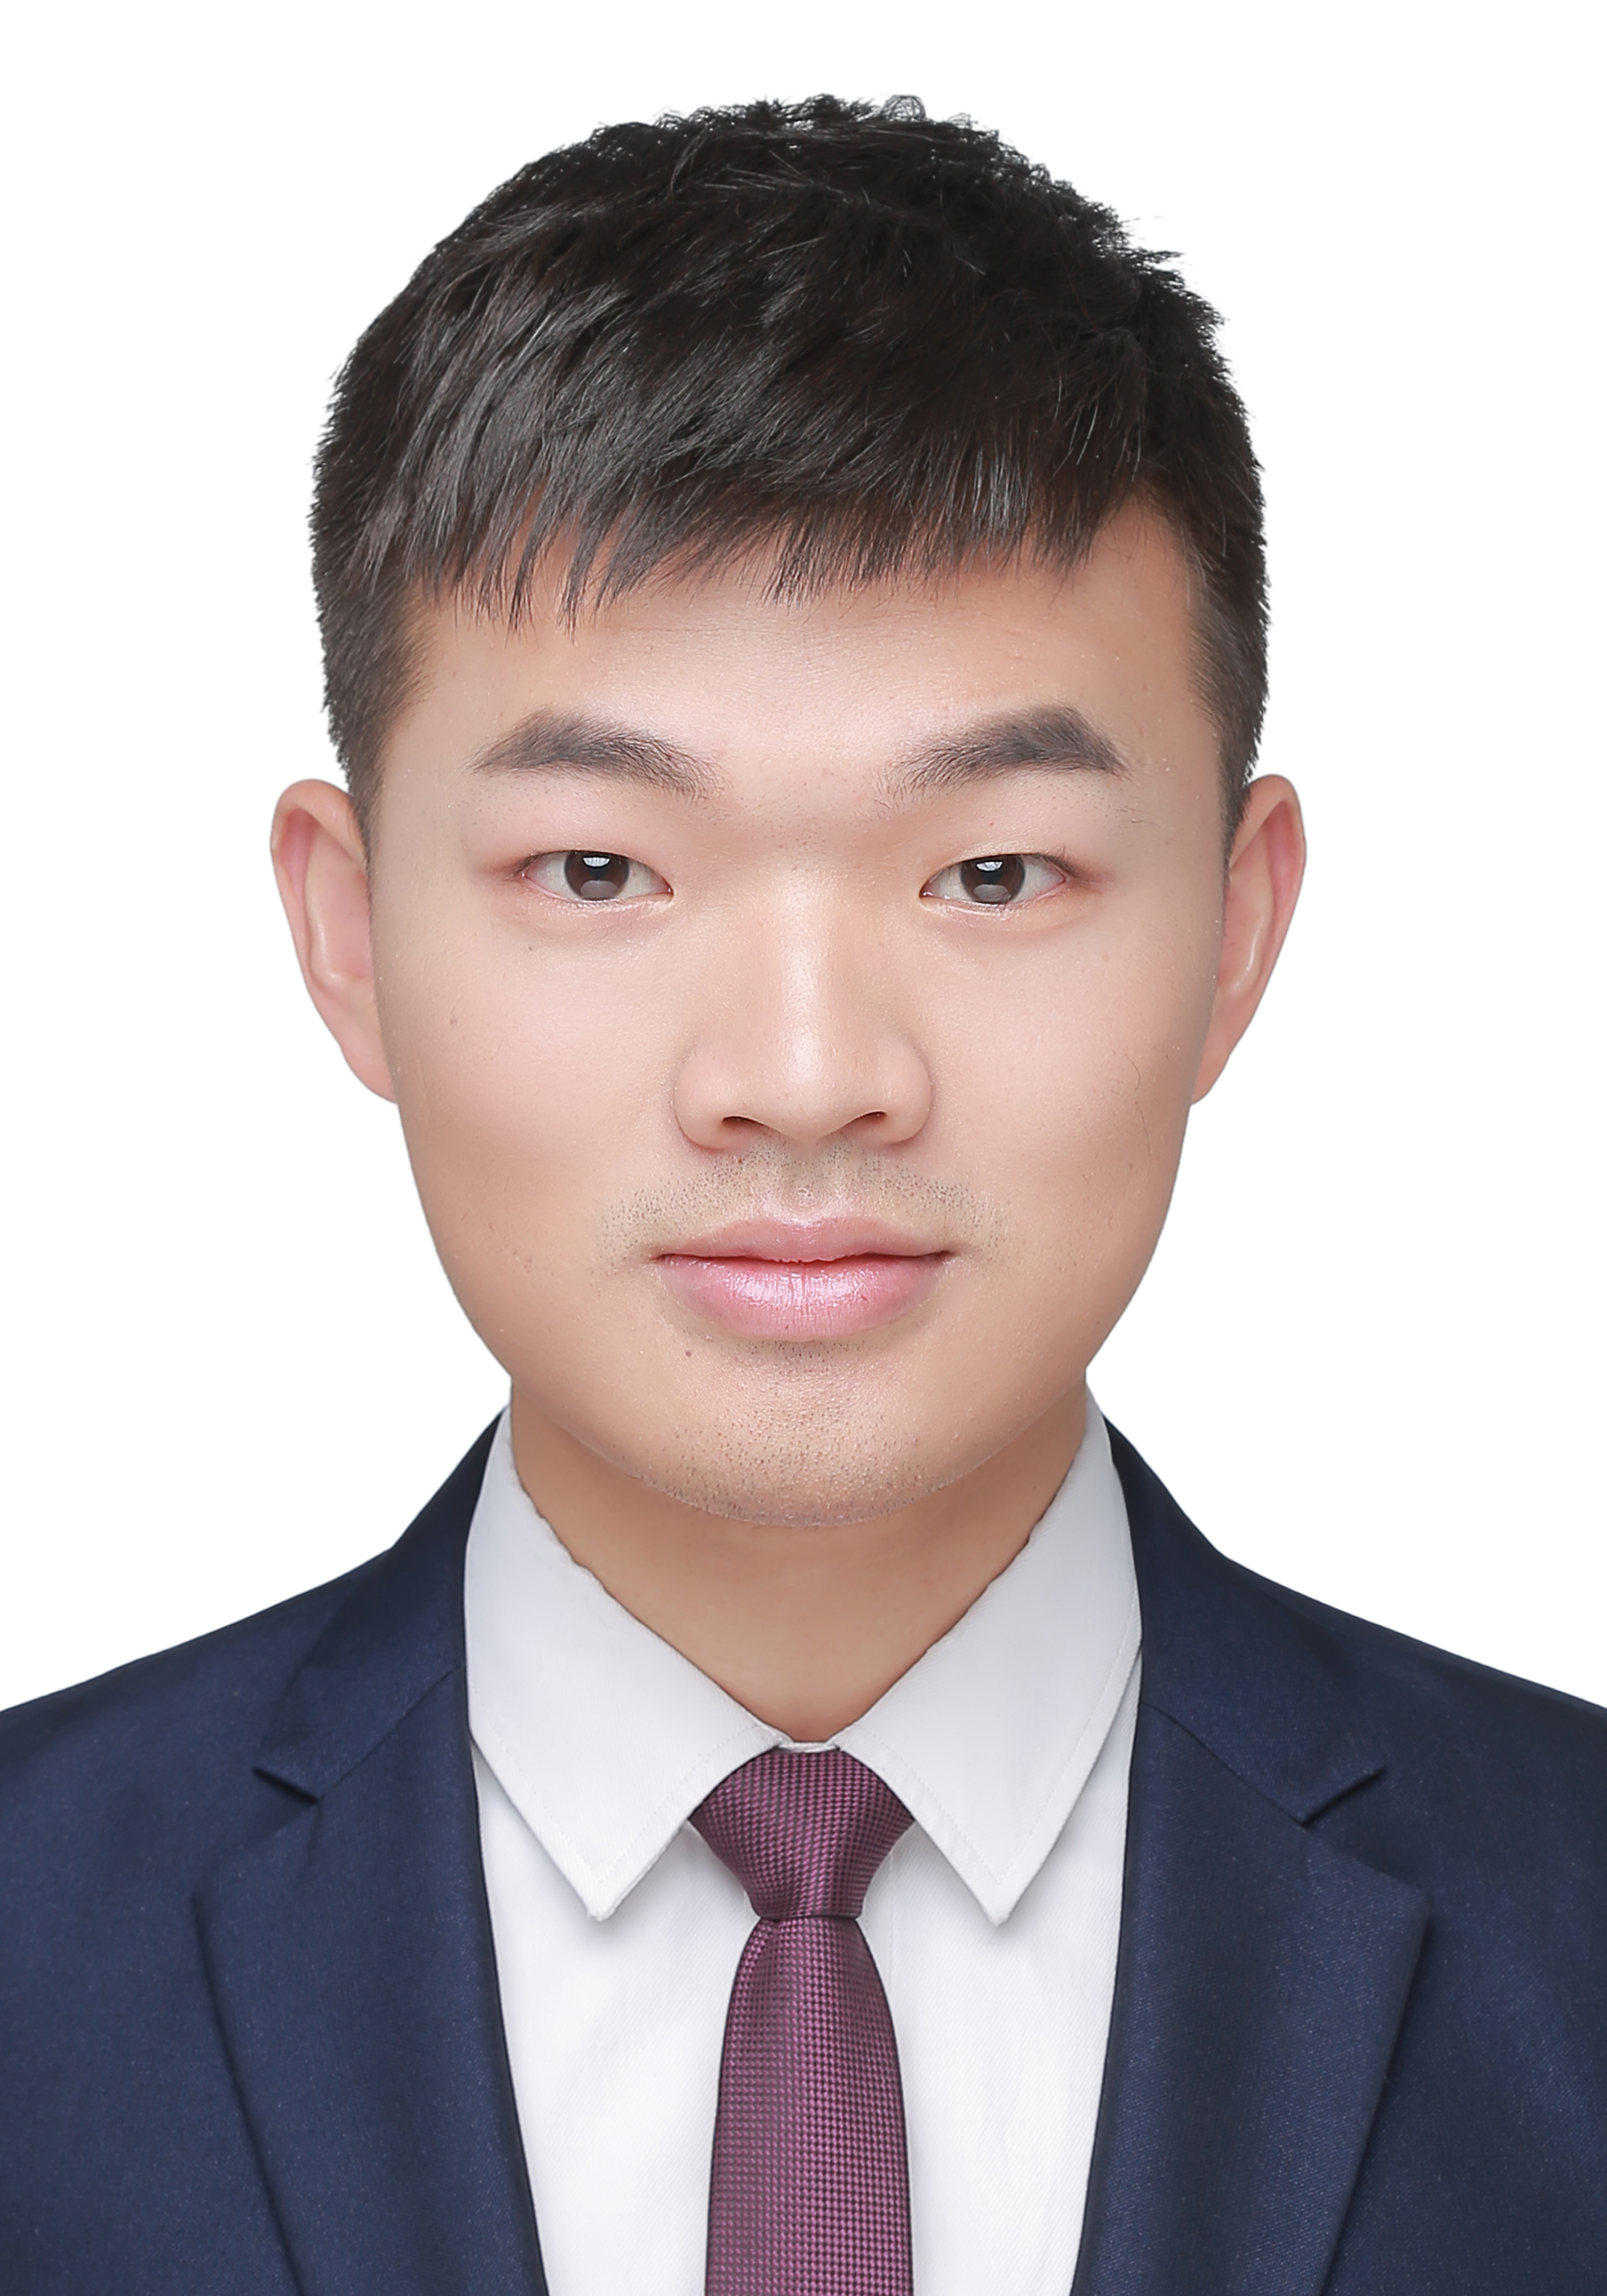
\includegraphics[width=0.88in]{avatar}
%             }
%             & \faBirthdayCake{1995.09.12} \\
%             & \phone{(+86)17600535912} \\
%             & \email{izhouwl@163.com} \\
%             & \homepage[www.zhouweilin.cn]{https://zhouweilin.cn} \\
%             & \github[github.com/Si3ver]{https://github.com/Si3ver} 
%         \end{tabu}
%     }
%     \columnbreak
%     \Large{
%         \begin{tabu}{ l l }
%             \multirow{5}{2.15in}{
%                 \name{周伟林}
%                 \basicInfo{
%                     \faSmileO{意向职位:web前端研发}
%                 }
%             }
%         \end{tabu}
%     }
% \end{multicols}

\begin{multicols}{4}
    \Large{
        \begin{tabu}{ r }
            \multirow{5}{1in}{
                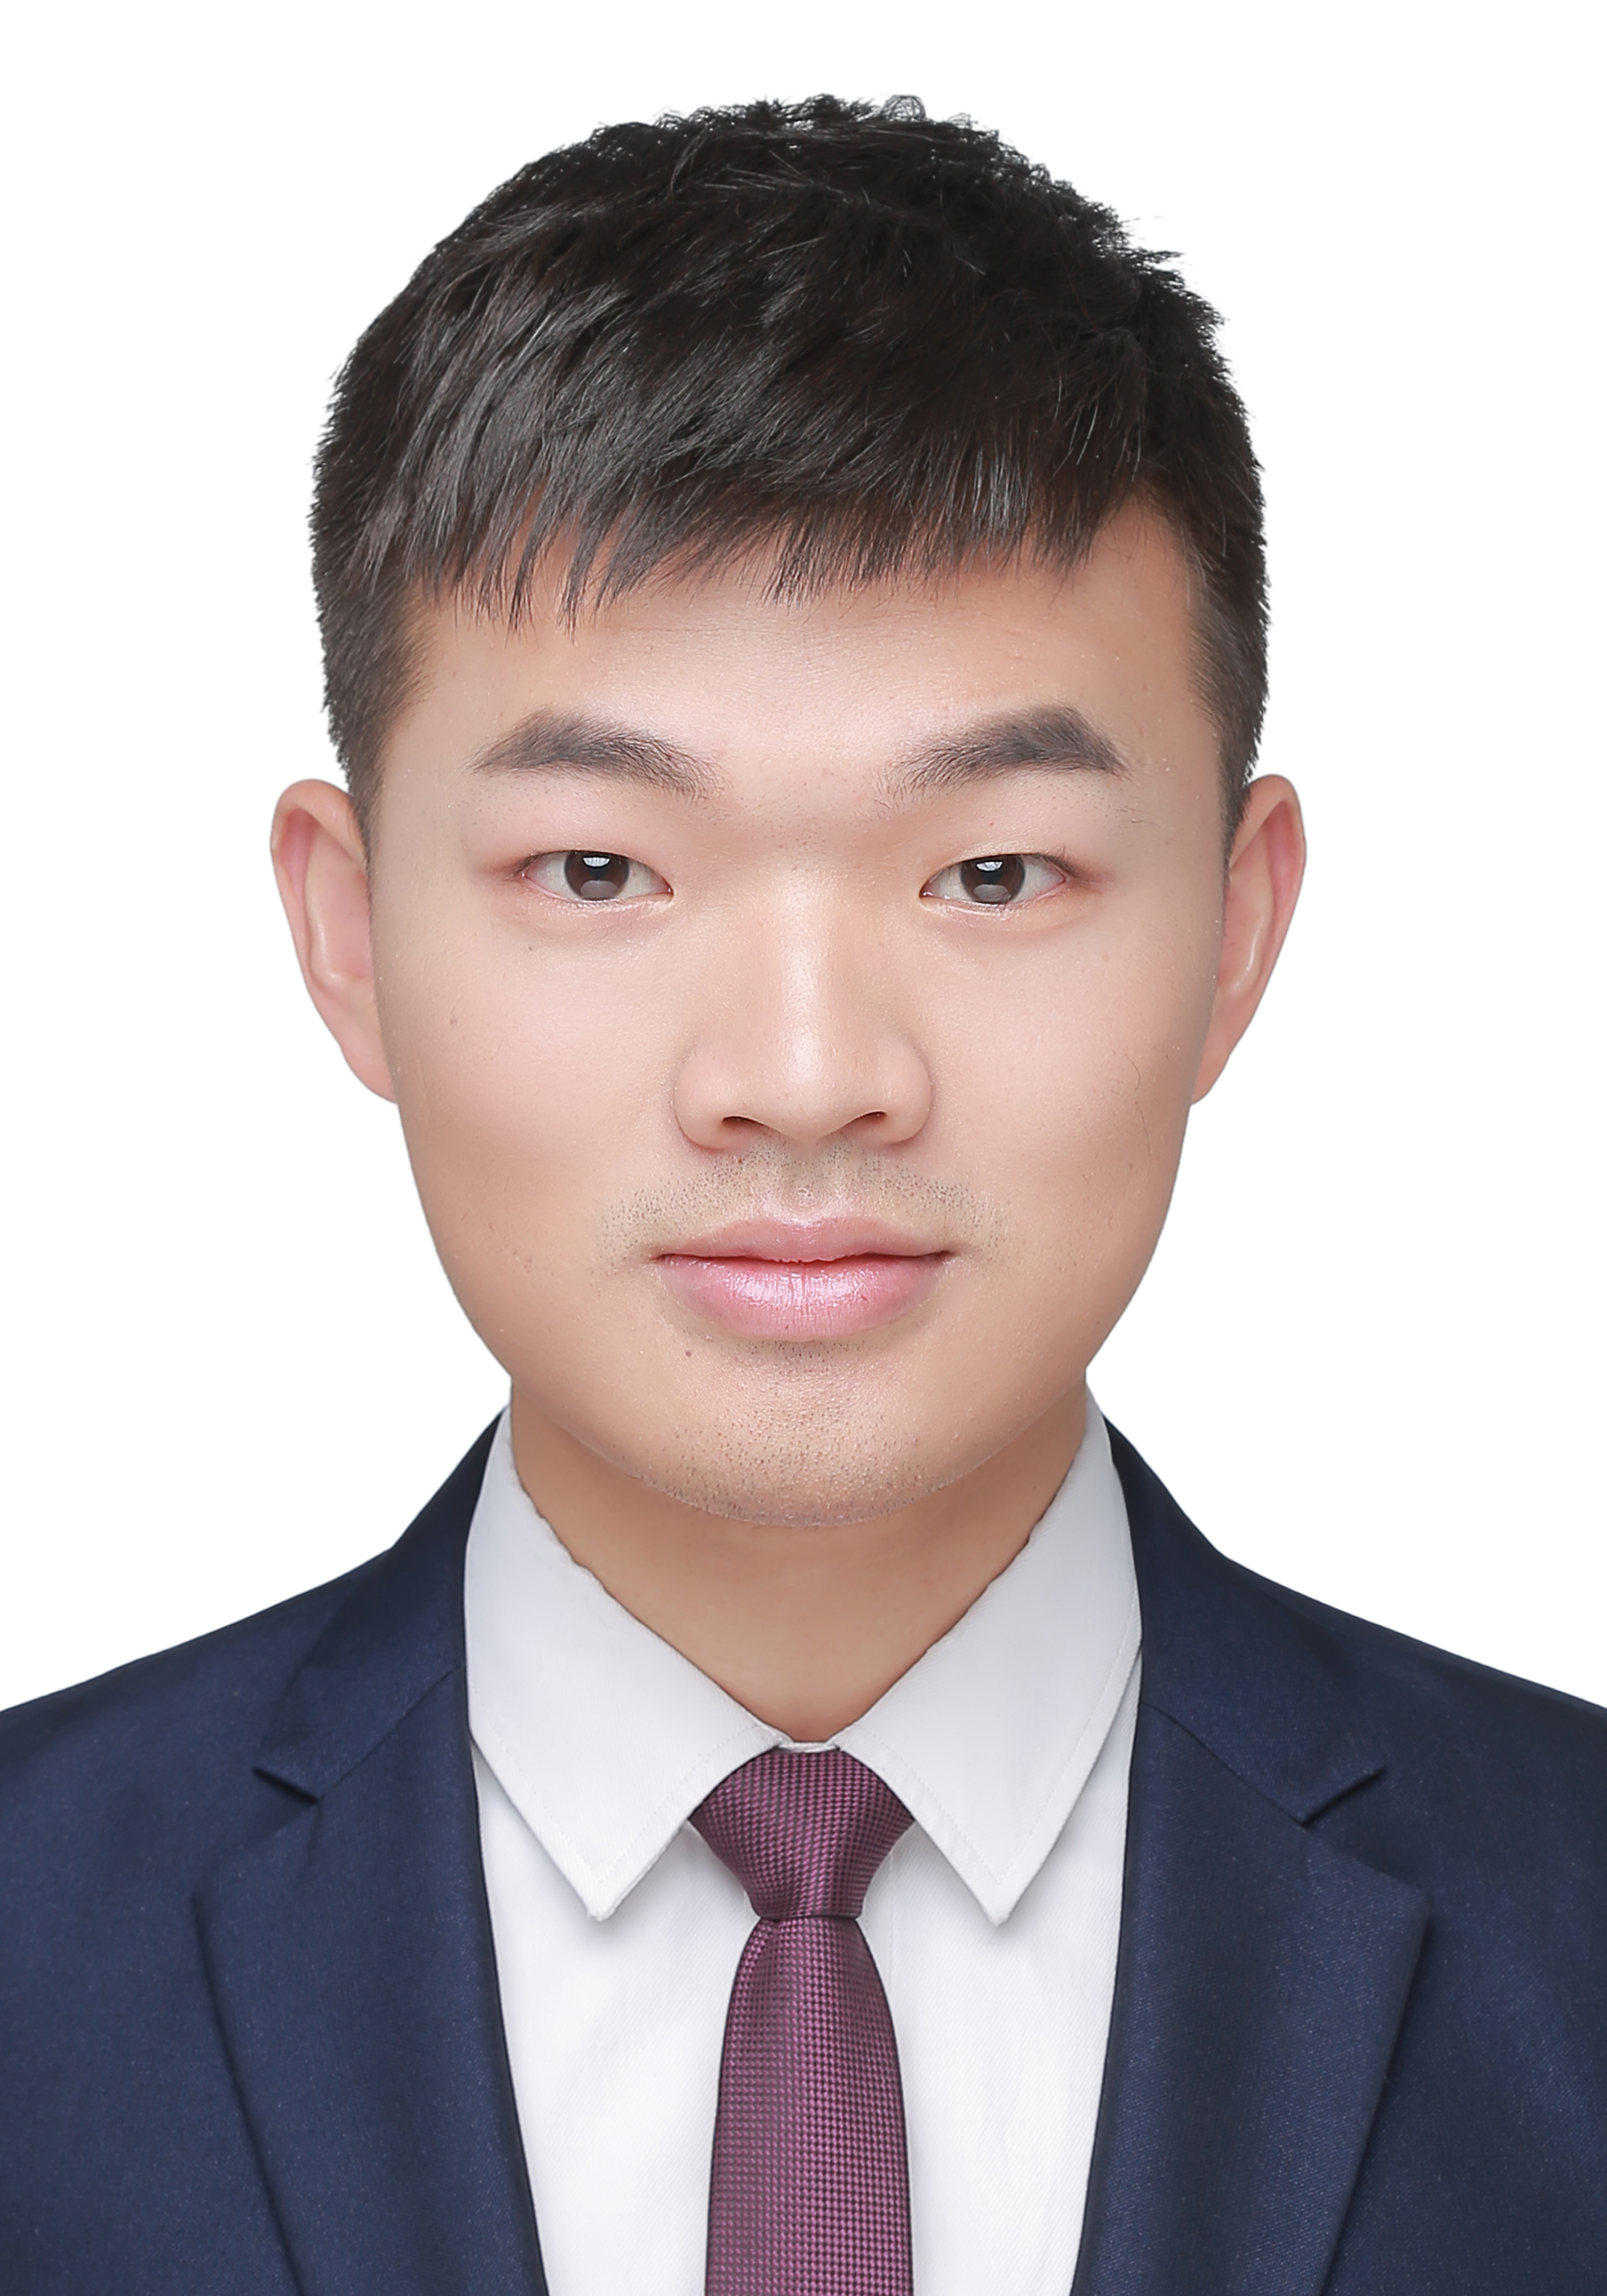
\includegraphics[width=0.88in]{avatar}
            }
        \end{tabu}
    }
    \columnbreak
    \Large{
        \begin{tabu}{ l l }
            & \faBirthdayCake{1995.09.12} \\
            & \phone{(+86)17600535912} \\
            & \email{izhouwl@163.com} \\
            & \homepage[\textbf{\color{red}{www.zhouweilin.cn}}]{https://zhouweilin.cn} \\
            & \github[github.com/Si3ver]{https://github.com/Si3ver} 
        \end{tabu}
    }
    \columnbreak
    \Large{
        \begin{tabu}{ r }
            \multirow{5}{3.5in}{
                \name{Weilin Zhou}
                \basicInfo{
                    \faSmileO{want job:software developer}
                }
            }
        \end{tabu}
    }
\end{multicols}

% 教育背景
\section{\faGraduationCap\  Education}
\datedsubsection{\textbf{Beijing University of Posts and Telecommunications(211)\quad}{\quad\quad\quad\quad\quad\quad Sep.2016 -- Jun.2019 }}
{{ Major: Computer Science }{\quad\quad\quad\quad\quad\quad\quad\quad\quad\quad\quad\quad\quad\quad\quad\quad\quad\quad\quad Academic Degree: Master}}
\datedsubsection{\textbf{Beijing University of Technology(211)\quad}{\quad\quad\quad\quad\quad\quad\quad\quad\quad\quad\quad\quad\quad\quad Sep.2012 -- Jun.2016 }}
{{ Major: Infomation Security }{\quad\quad\quad\quad\quad\quad\quad\quad\quad\quad\quad\quad\quad\quad\quad\quad\quad Academic Degree: Bechelor}}

% 实习经历
\section{\faBriefcase\ Internship Experience}
\datedsubsection{\textbf{滴滴出行\quad\quad\quad\quad\quad} \textbf{质量技术部\quad\quad\quad}{ WEB前端研发}}{2018年06月 -- 2018年09月}
\begin{itemize}
    \item[\faFlagO] 参与月光宝盒(订单流量重放平台)和Omega(移动数据管理平台)两个项目的前端部分开发
    \item[\faFlagO] 项目前后端分离,确定API格式后,前端利用\textbf{\color{red}{Mock}}数据开发,本地联调,线上测试
    \item[\faFlagO] 主要使用原生JS编写,并使用\textbf{\color{red}{模板引擎Simplite}}、Less、jQuery、BootStrap、ECharts等工具
    \item[\faCode] 客服反馈处理页、启动崩溃分析列表页与详细页等页面的开发
    \item[\faCode] 功能开发,包括列表筛选过滤功能、语言切换功能等
    \item[\faCode] 使用ECharts库,为页面添加折线图、柱状图、饼图
    \item[\faCode] \textbf{\color{red}{代码重构}}。删除幽灵代码,拆分冗长代码,增加报错信息,与后端合作合并部分过于细分的API
    \item[\faCheck] 页面上线到正式系统中,供公司内部使用;提高代码可维护性和可重用性
\end{itemize}


\datedsubsection{\textbf{西门子中国\quad\quad\quad\quad} \textbf{新闻传播部\quad\quad\quad}{网站技术支持}}{2017年10月 -- 2018年03月}
\begin{itemize}
    \item[\faFlagO] 参与CMS内容迁移(官网新闻发布平台,从SharePoint迁移到AEM)项目
    \item[\faFlagO] 原系统由ASP页面构成,新系统基于H5,迁移需要重写部分布局和前端组件
    \item[\faCode] 开发Slider组件,用以展示最新图片及公司公开刊物,并通过iframe嵌入到原页面内
    \item[\faCode] 获取网站埋点数据的统计结果,整理每月PV/UV报表数据
    \item[\faCheck] 使用英文书面沟通,与老外口语交流;接触到大型新闻发布系统的运维
\end{itemize}

\datedsubsection{\textbf{北京江南天安科技\quad} \textbf{软件研发部\quad\quad\quad}{Windows程序开发}}{2015年07月 -- 2015年09月}
\begin{itemize}
    \item[\faFlagO] 密码机是公司的重要产品,本人参与一款UKey软件的\textbf{\color{red}{windows开发}}部分
    \item[\faCode] 参与云密码机的专用UKey初始化工具、双因子认证软件的PC客户端开发
    \item[\faCheck] 熟悉了windows程序设计,熟练了VS的调试工具;加深了对安全通信和密码学的理解
\end{itemize}

% % 项目经历
% \section{\faUsers\ 项目经历}
% % \datedsubsection{\textbf{SVNF\quad\quad\quad\quad\quad\quad\quad\quad}{VNF放置算法}}{2018年07月 -- 08月}
% \begin{onehalfspacing}
% \begin{itemize}
%     \item[\faFlagO] 本项目属于实验室研究项目,本人研究方向为网络功能虚拟化
%     % \item[\faFlagO] 本项目属于实验室研究项目,本人研究方向为网络功能虚拟化
%     % \item[\faFlagO] 本项目属于实验室研究项目,本人研究方向为网络功能虚拟化
% \end{itemize}
% \end{onehalfspacing}

% 技能树
\section{\faCogs\ Skills}

\begin{itemize}
    \item[\faCheck] 熟悉原生JavaScript,有\textbf{\color{red}{H5移动端小游戏}}开发经验,有\textbf{\color{red}{python}}基础
    \item[\faCheck] 熟悉前端工程化开发,能书写和修改Webpack配置
    \item[\faCheck] 熟悉常用工具/库,包括\textbf{\color{red}{React.js}}、Canvas、ECharts、Bootstrap、AntD、jQuery、
    \item[\faCheck] 熟悉网络安全,理解\textbf{\color{red}{HTTPS}},有防火墙配置经验和网络安全协议开发经验
    \item[\faCheck] 熟悉python可视化库Matplotlib、排版工具Markdown、\textbf{\color{red}{LaTex}}
    \item[\faCheck] 通过CET-6,无障碍阅读英文文档,熟练使用Google、Stack Overflow检索
\end{itemize}


% 个人荣誉
\section{\faHeartO\ Awards}

\trophy[Weilin Zhou, Y Yang,and M Xu, Accommodating dynamic traffic immediately: a VNF placement approach]{https://github.com/Si3ver/SVNF}

\trophy[周伟林, 杨芫, 徐明伟. 网络功能虚拟化技术研究综述. 计算机研究与发展, 2018, 55(4): 675-688]{http://crad.ict.ac.cn/CN/abstract/abstract3662.shtml}

\trophy[2015全国大学生网络技术大赛(思科网院杯),全国二等奖,排名第12]{http://www.catc.edu.cn/2015cup/news/19rr5gvqfnqk2.xhtml} 


% 自我评价
\section{\faInfo\ Self Evaluation}
热爱技术,拥抱变化,持续\textbf{\color{red}{阅读}}

计算机\textbf{\color{red}{网络基础好}},持续的自我驱动力和学习能力

\end{document}
